\section{Převodníky AD a DA}
- základní princip, blokové schéma, základní statické a dynamické parametry, úloha v řetězci zpracování dat.

\subsection{Základní princip}
Při zpracování analogového signálu je jednou z důležitých funkcí převod tohoto signálu z analogové podoby do číslicové a naopak jsou ADC a DAC velmi důležitými prvky jakéhokoli systému zpracovávajícího signál.
   \begin{figure}[h]
   \begin{center}
     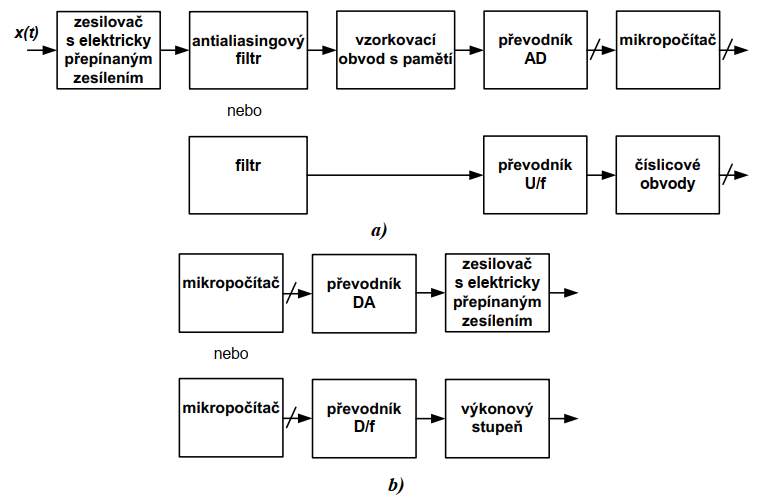
\includegraphics[scale=0.6]{images/ADCDAC.png}
   \end{center}
   \caption{Zařazení převodníku AD a DA v rámci měřicího přístroje}
  \end{figure}
  
Někdy je potřeba provádět měření na více vstupech nebo je nutné budit více výstupů. V těchto případech je pak nutno předřadit na vstup multiplexer a na výstup demultiplexer. 
Výstup je také obvykle doplněn o posilovač, který může být buď proudový, napěťový nebo obecně výkonový.  

Převodníky AD a DA jsou velmi důležitými stavebními prvky mnoha elektronických
zařízení. Obě skupiny převodníků mohou typicky obsahovat komparátory, číslicové obvody,
spínače, integrátory, vzorkovací obvody, přesný zdroj referenčního napětí a/nebo pasivní
součástky. Parametry převodníků lze rozdělit na statické (určují se z převodní charakteristiky)
a dynamické (určují se z kmitočtového spektra signálu)
\newpage
\subsection{Blokové schéma}
   \begin{figure}[h]
   \begin{center}
     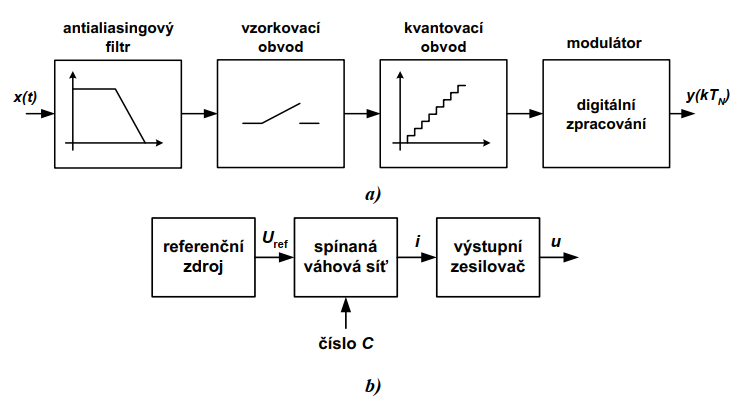
\includegraphics[scale=0.6]{images/Blok.png}
   \end{center}
   \caption{Blokové schéma a) ADC a b)DAC}
  \end{figure}
  
\subsection{Základní statické a dynamické parametry}
\textbf{Statické parametry} převodníků jsou určovány pomocí převodní charakteristiky.

\textbf{Dynamické vlastnosti} se vyhodnocují z kmitočtového spektra převodníku.

\textbf{Statické parametry}:
\begin{itemize}
\item rozsah,
\item integrální a diferenciální nelinearita (INL a DNL),
\item rozlišené převodníku (resolution),
\item přesnost (accuracy),
\item chyba monotónnosti,
\item chyba nastavení nuly (offset error),
\item a hysterze.
\end{itemize}

\textbf{Dynamické parametry}:
\begin{itemize}
\item odstup signál-šum (signal to noise ratio - SNR),
\item  efektivní počet bitů (effective number of bits - ENOB),
\item  harmonické zkreslení (total harmonic distortion - THD),
\item  odstup signál-šum a zkreslení (signal to noise and distortion - SINAD),
\item  dynamický rozsah bez parazitních složek (spurious free dynamic range - SFDR),
\item  krátké přechodové špičky (glitches),
\item  šum - vrcholový, efektivní (noise - rms, peak)
\item a doba přepnutí a ustálení a další.
\end{itemize}

\subsection{Úloha v řetězci zpracování dat}
Úloha v řetězci spočívá skoro vždy mezi senzorem zachycující data (teploměr, otáčkoměr, měření napětí...) a jednotkou, která tato data zpracovává (PC, MCU, FPGA...) v případě ADC. v případě DAC stojí v řetězci opět mezi jednotkou, která tentokrát posílá digitální data a např. reproduktorem, který přehrává analogový zvuk.






